Für die Sprache der korrekt geschachtelten Klammerausdrücke wurde in der
Vorlesung die Grammatik
\begin{equation}
\begin{aligned}
S\rightarrow
\texttt{(}S\texttt{)}
\;|\;
SS
\;|\;
\varepsilon
\label{40000052:grammar1}
\end{aligned}
\end{equation}
gefunden, die sich jedoch als nicht
eindeutig herausgestellt hat, das Wort \texttt{()} hat zum Beispiel die
beiden völlig verschiedenen Parse-Trees
\begin{center}
\def\l{1.5}
\def\h{1.2}
\def\pfeil#1#2{
	\draw[->,shorten <= 0.24cm,shorten >= 0.24cm] #1 -- #2;
}
\begin{tikzpicture}[>=latex,thick]
\coordinate (l0) at ({-3*\l},{0*\h});
\coordinate (r0) at ({3*\l},{0*\h});
\coordinate (l1) at ({-4*\l},{-1*\h});
\coordinate (l2) at ({-2*\l},{-1*\h});
\coordinate (r1) at ({4*\l},{-1*\h});
\coordinate (r2) at ({2*\l},{-1*\h});
\coordinate (l3) at ({-4*\l},{-2*\h});
\coordinate (l4) at ({-3*\l},{-2*\h});
\coordinate (l5) at ({-2*\l},{-2*\h});
\coordinate (l6) at ({-1*\l},{-2*\h});
\coordinate (r3) at ({4*\l},{-2*\h});
\coordinate (r6) at ({3*\l},{-2*\h});
\coordinate (r5) at ({2*\l},{-2*\h});
\coordinate (r4) at ({1*\l},{-2*\h});
\coordinate (l7) at ({-3*\l},{-3*\h});
\coordinate (l8) at ({-2*\l},{-3*\h});
\coordinate (l9) at ({-1*\l},{-3*\h});
\coordinate (r9) at ({3*\l},{-3*\h});
\coordinate (r8) at ({2*\l},{-3*\h});
\coordinate (r7) at ({1*\l},{-3*\h});
\pfeil{(l0)}{(l1)}
\pfeil{(l0)}{(l2)}
\pfeil{(l1)}{(l3)}
\pfeil{(l2)}{(l4)}
\pfeil{(l2)}{(l5)}
\pfeil{(l2)}{(l6)}
\pfeil{(l4)}{(l7)}
\pfeil{(l5)}{(l8)}
\pfeil{(l6)}{(l9)}
\node at (l0) {$S$};
\node at (l1) {$S$};
\node at (l2) {$S$};
\node at (l5) {$S$};
\node at (l4) {\texttt{(}};
\node at (l6) {\texttt{)}};
\node at (l7) {\texttt{(}};
\node at (l9) {\texttt{)}};
\node at (l3) {$\varepsilon$};
\pfeil{(r0)}{(r1)}
\pfeil{(r0)}{(r2)}
\pfeil{(r1)}{(r3)}
\pfeil{(r2)}{(r4)}
\pfeil{(r2)}{(r5)}
\pfeil{(r2)}{(r6)}
\pfeil{(r4)}{(r7)}
\pfeil{(r5)}{(r8)}
\pfeil{(r6)}{(r9)}
\node at (r0) {$S$};
\node at (r1) {$S$};
\node at (r2) {$S$};
\node at (r5) {$S$};
\node at (r4) {\texttt{(}};
\node at (r6) {\texttt{)}};
\node at (r7) {\texttt{(}};
\node at (r9) {\texttt{)}};
\node at (r3) {$\varepsilon$};
\end{tikzpicture}
\end{center}


Betrachten Sie die Grammatik
\begin{equation}
\begin{aligned}
S&\rightarrow \texttt{(} S \texttt{)} S
\\
&\rightarrow \varepsilon
\end{aligned}
\label{40000052:grammar2}
\end{equation}
\begin{teilaufgaben}
\item Finden Sie den Parse Tree von \texttt{()} in der Grammatik
\eqref{40000052:grammar2}.
\item Ist die Grammatik \eqref{40000052:grammar2} eindeutig?
\item Finden Sie die Chomsky-Normalform dieser Grammatik.
\end{teilaufgaben}

\thema{Grammatik}
\thema{Parse Tree}
\thema{eindeutiger Parse Tree}
\thema{Chomsky Normalform}

\begin{loesung}
\begin{teilaufgaben}
\item Der Parse Tree ist
\begin{center}
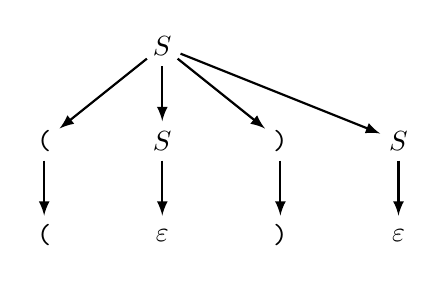
\begin{tikzpicture}[>=latex,thick]
\def\l{1.5}
\def\h{1.2}
\def\pfeil#1#2{
	\draw[->,shorten >= 0.25cm,shorten <= 0.25cm] #1 -- #2;
}
\coordinate (q0) at (0,0);
\coordinate (q1) at ({-1*\l},{-1*\h});
\coordinate (q2) at ({0*\l},{-1*\h});
\coordinate (q3) at ({1*\l},{-1*\h});
\coordinate (q4) at ({2*\l},{-1*\h});
\coordinate (q5) at ({-1*\l},{-2*\h});
\coordinate (q6) at ({0*\l},{-2*\h});
\coordinate (q7) at ({1*\l},{-2*\h});
\coordinate (q8) at ({2*\l},{-2*\h});
\node at (q0) {$S$};
\node at (q2) {$S$};
\node at (q4) {$S$};
\node at (q1) {\texttt{(}};
\node at (q5) {\texttt{(}};
\node at (q3) {\texttt{)}};
\node at (q7) {\texttt{)}};
\node at (q6) {$\varepsilon$};
\node at (q8) {$\varepsilon$};
\pfeil{(q0)}{(q1)}
\pfeil{(q0)}{(q2)}
\pfeil{(q0)}{(q3)}
\pfeil{(q0)}{(q4)}
\pfeil{(q1)}{(q5)}
\pfeil{(q2)}{(q6)}
\pfeil{(q3)}{(q7)}
\pfeil{(q4)}{(q8)}
\end{tikzpicture}
\end{center}
\item Die Grammatik ist eindeutig, weil für jede öffnende Klammer die erste 
Regel genau einmal angewendet werden muss. 
Die Grammatik
\eqref{40000052:grammar1} dagegen lässt immer die Option offen, die
Regel $S\to SS$ anzuwenden, was zur Zweideutigkeit führt.
\item Zunächst muss sichergestellt werden, dass die Startvariable auf
der rechten Seite nicht vorkommt:
\begin{align*}
S_0&\rightarrow S
\\
S&\rightarrow \texttt{(} S \texttt{)} S \;|\; \varepsilon
\end{align*}
Jetzt müssen $\varepsilon$-Regeln entfernt werden:
\begin{align*}
S_0&\rightarrow
S
\;|\;
\varepsilon
\\
S&\rightarrow
\texttt{(} S \texttt{)} S \;|\;
\texttt{(}  \texttt{)} S \;|\;
\texttt{(} S \texttt{)}  \;|\;
\texttt{(}  \texttt{)} 
\end{align*}
Jetzt müssen Unit-Rules entfernt werden:
\begin{align*}
S_0&\rightarrow
\texttt{(} S \texttt{)} S \;|\;
\texttt{(}  \texttt{)} S \;|\;
\texttt{(} S \texttt{)}  \;|\;
\texttt{(}  \texttt{)} 
\;|\;
\varepsilon
\\
S&\rightarrow
\texttt{(} S \texttt{)} S \;|\;
\texttt{(}  \texttt{)} S \;|\;
\texttt{(} S \texttt{)}  \;|\;
\texttt{(}  \texttt{)} 
\end{align*}
Jetzt müssen nur noch die verbleibenden Sequenzen aufgeteilt werden:
\begin{align*}
S_0&\rightarrow
AX \;|\;
AY \;|\;
AZ  \;|\;
AB 
\;|\;
\varepsilon
\\
S&\rightarrow
AX \;|\;
AY \;|\;
AZ  \;|\;
AB 
\\
A&\rightarrow \texttt{(}\\
B&\rightarrow \texttt{)}\\
X&\rightarrow SY \\
Y&\rightarrow BS \\
Z&\rightarrow SB
\end{align*}
Damit ist Chomsky-Normalform erreicht.
\qedhere
\end{teilaufgaben}
\end{loesung}

\begin{bewertung}
\begin{teilaufgaben}
\item
Parse Tree ({\bf P}) 1 Punkt.
\item
Begründung für Eindeutigkeit ({\bf B})  1 Punkt.
\item
Startvariable nur auf der linken Seite ({\bf S}) 1 Punkt,
Epsilon-Regel ({\bf E}) 1 Punkt,
Unit-Rules ({\bf U}) 1 Punkt,
Mehrfach-Regeln und Terminalsymbole ({\bf T}) 1 Punkt.
\end{teilaufgaben}
\end{bewertung}




